\documentclass{csbeamer}

\usepackage{dsfont}
\usepackage{amsmath}
\usepackage{amssymb}
\usepackage{algorithm}
\usepackage{algpseudocode}
\usepackage{pgfplots}
\usepackage{colortbl}
\usepackage{xcolor}
\pgfplotsset{compat=1.18}

% Add custom color definitions for On-Policy Prediction
\definecolor{approxmain}{HTML}{1565C0}
\definecolor{approxaccent}{HTML}{FF7043}
\definecolor{approxlight}{HTML}{42A5F5}
\definecolor{approxsecondary}{HTML}{8E24AA}
\definecolor{gradientcolor}{HTML}{388E3C}
\definecolor{neuralcolor}{HTML}{FF5722}
\definecolor{linearcolor}{HTML}{2196F3}
\definecolor{statecolor}{HTML}{9C27B0}
\definecolor{weightcolor}{HTML}{795548}
\definecolor{errorcolor}{HTML}{D32F2F}
\definecolor{targetcolor}{HTML}{4CAF50}
\definecolor{featurecolor}{HTML}{FF9800}

\university{St. Francis Xavier University}
\department{Department of Computer Science}
\course{CSCI-531 - Reinforcement Learning}
\courseshort{CSCI-531 - RL}
\term{Fall 2025}
\author{Dr. Jean-Alexis Delamer}

\title{Approximation - On-Policy Prediction}

\begin{document}

\frame{\titlepage}

% Section: Introduction to Approximation
\section{From Tabular to Approximation}

\subsection{Limitations of Tabular Methods}

\begin{frame}
    \frametitle{The Tabular Method Approach}

    \begin{block}<1->{What are Tabular Methods?}
        \begin{itemize}
            \item<1-> Store \textcolor{approxmain}{\textbf{exact value}} $q_\pi(s,a)$ for \textcolor{approxaccent}{\textbf{each}} state-action pair
            \item<2-> Create a \textcolor{statecolor}{\textbf{lookup table}} with all possible combinations
            \item<3-> Perfect representation when feasible
        \end{itemize}
    \end{block}

    \begin{center}
        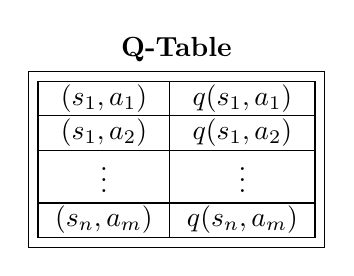
\begin{tikzpicture}[scale=0.8]
            \node[draw, rectangle, minimum width=3cm, minimum height=2cm] (table) at (0,0) {
                \begin{tabular}{|c|c|}
                    \hline
                    $(s_1,a_1)$ & $q(s_1,a_1)$ \\
                    \hline
                    $(s_1,a_2)$ & $q(s_1,a_2)$ \\
                    \hline
                    $\vdots$ & $\vdots$ \\
                    \hline
                    $(s_n,a_m)$ & $q(s_n,a_m)$ \\
                    \hline
                \end{tabular}
            };
            \node[above] at (table.north) {\textbf{Q-Table}};
        \end{tikzpicture}
    \end{center}

    \visible<4->{
        \begin{alertblock}{Activity}
            What issues can arise with this approach for large state spaces?
        \end{alertblock}
    }
\end{frame}

\begin{frame}
    \frametitle{Problems with Tabular Methods}

    \begin{block}<1->{Scalability Issues}
        \begin{itemize}
            \item<1-> \textcolor{errorcolor}{\textbf{Memory explosion}}: Space complexity $O(|S| \times |A|)$
            \item<2-> \textcolor{errorcolor}{\textbf{Learning time}}: Need to visit every state-action pair
            \item<3-> \textcolor{errorcolor}{\textbf{Generalization}}: No knowledge transfer between similar states
        \end{itemize}
    \end{block}

    \begin{block}<4->{Real-World Examples}
        \begin{itemize}
            \item<4-> \textbf{Chess}: $\approx 10^{47}$ possible positions
            \item<5-> \textbf{Atari games}: $256^{84 \times 84} \approx 10^{170,000}$ pixel combinations
            \item<6-> \textbf{Autonomous driving}: Continuous sensor readings
        \end{itemize}
    \end{block}

    \visible<7->{
        \begin{center}
            \textcolor{approxmain}{\textbf{Solution}: Function Approximation}
        \end{center}
    }
\end{frame}

% Section: Value Function Approximation
\section{Value Function Approximation}

\subsection{The Weight Vector Approach}

\begin{frame}
    \frametitle{The Fundamental Shift: Tables vs Functions}

    \begin{block}<1->{Tabular Method (What We've Done Before)}
        \begin{itemize}
            \item<1-> \textbf{One number per state}: Store $v(s_1), v(s_2), \ldots, v(s_n)$
            \item<2-> \textbf{Independent values}: Updating $v(s_1)$ doesn't affect $v(s_2)$
            \item<3-> \textbf{Perfect but expensive}: Exact values but need $|S|$ memory slots
        \end{itemize}
    \end{block}

    \begin{center}
        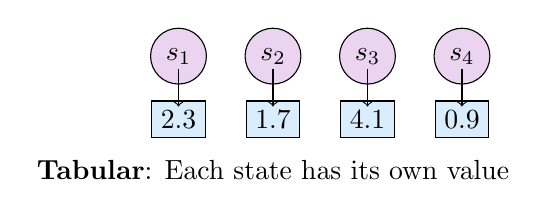
\begin{tikzpicture}[scale=0.8]
            % States
            \foreach \i/\val in {1/2.3, 2/1.7, 3/4.1, 4/0.9} {
                \node[draw, circle, fill=statecolor!20] at (\i*1.5-1,1) {$s_\i$};
                \node[draw, rectangle, fill=approxlight!20] at (\i*1.5-1,0) {$\val$};
                \draw[->] (\i*1.5-1,0.8) -- (\i*1.5-1,0.2);
            }
            \node[below] at (2,-0.5) {\textbf{Tabular}: Each state has its own value};
        \end{tikzpicture}
    \end{center}

    \visible<4->{
        \begin{alertblock}{The Problem}
            What if we have 1 million states? We need 1 million separate values!
        \end{alertblock}
    }
\end{frame}

\begin{frame}
    \frametitle{Function Approximation: The Core Idea}

    \begin{block}<1->{Key Innovation}
        Instead of storing individual values, use a \textcolor{approxmain}{\textbf{function}} with \textcolor{weightcolor}{\textbf{parameters}}
    \end{block}

    \begin{center}
        \begin{tikzpicture}[scale=0.8]
            % Weight vector
            \node[draw, rectangle, fill=weightcolor!20, minimum width=2cm, minimum height=1cm] (w) at (0,2) {
                $\mathbf{w} = \begin{bmatrix} w_1 \\ w_2 \\ w_3 \end{bmatrix}$
            };

            % Function
            \node[draw, ellipse, fill=neuralcolor!20] (func) at (0,0) {$\hat{v}(s,\mathbf{w})$};

            % Arrow from weights to function
            \draw[->, thick] (w) -- (func);

            % States and their computed values
            \foreach \i/\s in {1/s_1, 2/s_2, 3/s_3, 4/s_4} {
                \node[draw, circle, fill=statecolor!20] at (\i*2-5,-2) {$\s$};
                \draw[->] (func) -- (\i*2-5,-1.3);
                \node[below] at (\i*2-5,-2.5) {\small $\hat{v}(\s,\mathbf{w})$};
            }

            \node[right] at (2,2) {\textcolor{weightcolor}{\textbf{3 parameters}}};
            \node[right] at (2,-2) {\textbf{Infinite states possible!}};
        \end{tikzpicture}
    \end{center}
\end{frame}

\begin{frame}
    \frametitle{Why Function Approximation Works}

    \begin{block}<1->{The Magic of Shared Parameters}
        \begin{itemize}
            \item<1-> \textcolor{approxaccent}{\textbf{Shared parameters}}: Same $\mathbf{w}$ computes values for ALL states
            \item<2-> \textcolor{approxmain}{\textbf{Generalization}}: Similar states get similar values automatically
            \item<3-> \textcolor{targetcolor}{\textbf{Efficiency}}: Store only $d$ parameters instead of $|S|$ values
        \end{itemize}
    \end{block}

    \begin{block}<4->{Key Benefits}
        \begin{itemize}
            \item<4-> \textbf{Memory savings}: $d \ll |S|$ means huge space reduction
            \item<5-> \textbf{Learning transfer}: Knowledge about one state helps with similar states
            \item<6-> \textbf{Handles continuous spaces}: Can work with infinite state spaces
        \end{itemize}
    \end{block}

    \visible<7->{
        \begin{alertblock}{Trade-off}
            We gain efficiency and generalization, but lose the guarantee of exact values
        \end{alertblock}
    }
\end{frame}

\begin{frame}
    \frametitle{Concrete Example: GridWorld}

    \begin{block}<1->{Scenario: 4×4 GridWorld (16 states)}
        \textbf{Tabular}: Need 16 separate values \\
        \textbf{Function Approximation}: Maybe just 3 parameters!
    \end{block}

    \begin{columns}
        \begin{column}{0.45\textwidth}
            \begin{center}
                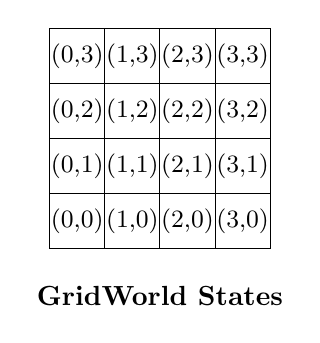
\begin{tikzpicture}[scale=0.7]
                    % Grid
                    \foreach \x in {0,1,2,3} {
                        \foreach \y in {0,1,2,3} {
                            \draw (\x,\y) rectangle (\x+1,\y+1);
                            \node at (\x+0.5,\y+0.5) {\small (\x,\y)};
                        }
                    }
                    \node[below] at (2,-0.5) {\textbf{GridWorld States}};
                \end{tikzpicture}
            \end{center}
        \end{column}

        \begin{column}{0.55\textwidth}
            \begin{center}
                \textbf{Function:} \\
                $\hat{v}(x,y,\mathbf{w}) = w_1 \cdot x + w_2 \cdot y + w_3$

                \vspace{0.5cm}

                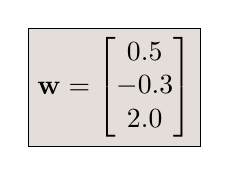
\begin{tikzpicture}[scale=0.8]
                    \node[draw, rectangle, fill=weightcolor!20] at (0,0) {
                        $\mathbf{w} = \begin{bmatrix} 0.5 \\ -0.3 \\ 2.0 \end{bmatrix}$
                    };
                \end{tikzpicture}

                \vspace{0.3cm}

                {\small
                \begin{tabular}{l}
                    $\hat{v}(0,0) = 0.5(0) + (-0.3)(0) + 2.0 = 2.0$ \\
                    $\hat{v}(1,0) = 0.5(1) + (-0.3)(0) + 2.0 = 2.5$ \\
                    $\hat{v}(3,3) = 0.5(3) + (-0.3)(3) + 2.0 = 2.6$
                \end{tabular}
                }
            \end{center}
        \end{column}
    \end{columns}
\end{frame}

\begin{frame}
    \frametitle{Concrete Example: GridWorld}
    \begin{columns}
        \begin{column}{0.45\textwidth}
            \begin{center}
                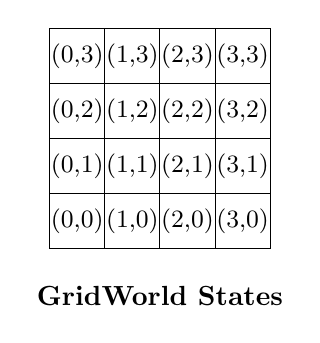
\begin{tikzpicture}[scale=0.7]
                    % Grid
                    \foreach \x in {0,1,2,3} {
                        \foreach \y in {0,1,2,3} {
                            \draw (\x,\y) rectangle (\x+1,\y+1);
                            \node at (\x+0.5,\y+0.5) {\small (\x,\y)};
                        }
                    }
                    \node[below] at (2,-0.5) {\textbf{GridWorld States}};
                \end{tikzpicture}
            \end{center}
        \end{column}

        \begin{column}{0.55\textwidth}
            \begin{center}
                \textbf{Function:} \\
                $\hat{v}(x,y,\mathbf{w}) = w_1 \cdot x + w_2 \cdot y + w_3$

                \vspace{0.5cm}

                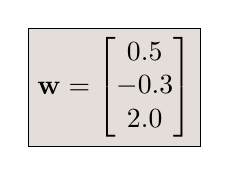
\begin{tikzpicture}[scale=0.8]
                    \node[draw, rectangle, fill=weightcolor!20] at (0,0) {
                        $\mathbf{w} = \begin{bmatrix} 0.5 \\ -0.3 \\ 2.0 \end{bmatrix}$
                    };
                \end{tikzpicture}

                \vspace{0.3cm}

                {\small
                \begin{tabular}{l}
                    $\hat{v}(0,0) = 0.5(0) + (-0.3)(0) + 2.0 = 2.0$ \\
                    $\hat{v}(1,0) = 0.5(1) + (-0.3)(0) + 2.0 = 2.5$ \\
                    $\hat{v}(3,3) = 0.5(3) + (-0.3)(3) + 2.0 = 2.6$
                \end{tabular}
                }
            \end{center}
        \end{column}
    \end{columns}

    \visible<2->{
        \begin{alertblock}{Key Insight}
            Changing $w_1$ affects the value of \textcolor{errorcolor}{\textbf{all}} states. This is both powerful and challenging.
        \end{alertblock}
    }
\end{frame}

\subsection{Update Notation and Targets}

\begin{frame}
    \frametitle{Update Targets in Approximation}

    \begin{block}<1->{General Update Form}
        \begin{center}
            \textcolor{approxmain}{$NewEstimate \leftarrow OldEstimate + StepSize[Target - OldEstimate]$}
        \end{center}
    \end{block}

    \begin{columns}
        \begin{column}{0.5\textwidth}
            \begin{block}<2->{Update Notation: $s \mapsto u$}
                \begin{itemize}
                    \item<2-> $s$: The state being updated
                    \item<3-> $u$: The \textcolor{targetcolor}{\textbf{target value}} for that state
                \end{itemize}
            \end{block}

            \visible<7->{
                \begin{center}
                    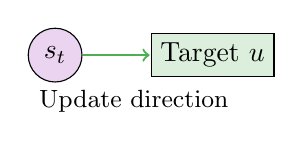
\begin{tikzpicture}[scale=0.8]
                        \node[draw, circle, fill=statecolor!20] (state) at (0,0) {$s_t$};
                        \draw[->, thick, targetcolor] (state) -- (1.5,0);
                        \node[draw, rectangle, fill=targetcolor!20] (target) at (2.5,0) {Target $u$};
                        \node[below] at (1.25,-0.4) {\small Update direction};
                    \end{tikzpicture}
                \end{center}
            }
        \end{column}

        \begin{column}{0.5\textwidth}
            \begin{block}<4->{Method-Specific Targets}
                \begin{itemize}
                    \item<4-> \textbf{Monte Carlo}: $s_t \mapsto G_t$ (return)
                    \item<5-> \textbf{TD(0)}: $s_t \mapsto r_{t+1} + \gamma\hat{v}(s_{t+1}, \mathbf{w})$
                    \item<6-> \textbf{n-step TD}: $s_t \mapsto G_{t:t+n}$
                \end{itemize}
            \end{block}
        \end{column}
    \end{columns}
\end{frame}

\begin{frame}
    \frametitle{The Generalization Challenge}

    \begin{alertblock}<1->{Key Problem}
        Updating one state affects the approximation for \textcolor{errorcolor}{\textbf{all other states}}!
    \end{alertblock}

    \begin{columns}
        \begin{column}{0.5\textwidth}
            \begin{center}
                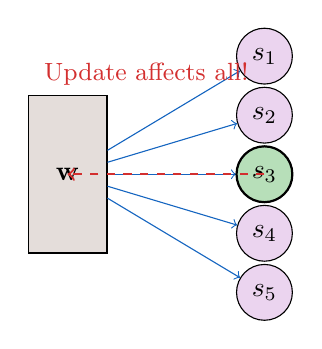
\begin{tikzpicture}
                    % Weight vector
                    \node[draw, rectangle, fill=weightcolor!20, minimum width=1cm, minimum height=2cm] (w) at (0,0) {$\mathbf{w}$};

                    % Multiple states
                    \foreach \i/\y in {1/1.5, 2/0.75, 3/0, 4/-0.75, 5/-1.5} {
                        \node[draw, circle, fill=statecolor!20] (s\i) at (2.5,\y) {$s_\i$};
                        \draw[->, approxmain] (w) -- (s\i);
                    }

                    % Highlight one state being updated
                    \node[draw, circle, fill=targetcolor!40, thick] at (2.5,0) {$s_3$};
                    \draw[->, thick, errorcolor, dashed] (2.5,0) -- (0,0);
                    \node[above, errorcolor] at (1,1) {\small Update affects all!};
                \end{tikzpicture}
            \end{center}
        \end{column}

        \begin{column}{0.5\textwidth}
            \begin{block}<2->{Consequence}
                \begin{itemize}
                    \item<2-> Making one state's estimate \textcolor{targetcolor}{\textbf{more accurate}}
                    \item<3-> Invariably makes others' \textcolor{errorcolor}{\textbf{less accurate}}
                    \item<4-> Need to prioritize which states matter most
                \end{itemize}
            \end{block}
        \end{column}
    \end{columns}
\end{frame}

% Section: Prediction Objective
\section{Prediction Objective}

\subsection{State Distribution and Importance}

\begin{frame}
    \frametitle{Defining State Importance}

    \begin{block}<1->{State Distribution $\mu(s)$}
        \begin{itemize}
            \item<1-> $\mu(s) \geq 0$ for all states $s$
            \item<2-> $\sum_{s} \mu(s) = 1$ (probability distribution)
            \item<3-> \textcolor{approxaccent}{\textbf{Higher}} $\mu(s)$ = \textcolor{approxaccent}{\textbf{more important}} state
        \end{itemize}
    \end{block}

    \begin{center}
        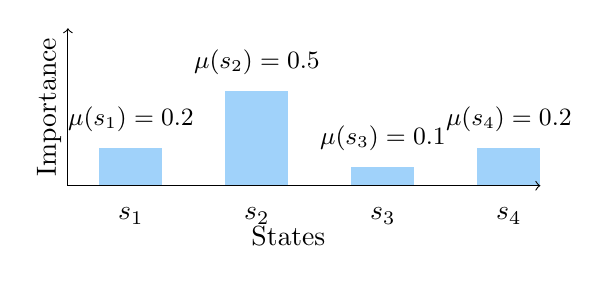
\begin{tikzpicture}[scale=0.8]
            % States with different importance
            \foreach \x/\s/\h in {0/s_1/0.2, 2/s_2/0.5, 4/s_3/0.1, 6/s_4/0.2} {
                \fill[approxlight!50] (\x,0) rectangle (\x+1,\h*3);
                \node[below] at (\x+0.5,-0.2) {$\s$};
                \node[above] at (\x+0.5,\h*3+0.1) {\small $\mu(\s)=\h$};
            }
            \draw[->] (-0.5,0) -- (7,0);
            \draw[->] (-0.5,0) -- (-0.5,2.5);
            \node[below] at (3,-0.5) {States};
            \node[left, rotate=90] at (-0.8,2.5) {Importance};
        \end{tikzpicture}
    \end{center}

\end{frame}

\begin{frame}
    \frametitle{Defining State Importance}

    \begin{block}{State Distribution $\mu(s)$}
        \begin{itemize}
            \item $\mu(s) \geq 0$ for all states $s$
            \item $\sum_{s} \mu(s) = 1$ (probability distribution)
            \item \textcolor{approxaccent}{\textbf{Higher}} $\mu(s)$ = \textcolor{approxaccent}{\textbf{more important}} state
        \end{itemize}
    \end{block}

    \begin{block}<2->{Common Choice: On-Policy Distribution}
        \begin{itemize}
            \item<2-> $\mu(s) = $ fraction of time spent in state $s$ under policy $\pi$
            \item<3-> Focus learning on \textcolor{approxmain}{\textbf{frequently visited}} states
        \end{itemize}
    \end{block}
\end{frame}

\subsection{Mean Squared Value Error}

\begin{frame}
    \frametitle{The Objective Function}

    \begin{block}<1->{Mean Squared Value Error (MSVE)}
        \begin{align}
            \textcolor{errorcolor}{\overline{\text{VE}}(\mathbf{w})} &= \sum_{s \in S} \mu(s) \left[ v_\pi(s) - \hat{v}(s,\mathbf{w}) \right]^2
        \end{align}
    \end{block}

    \begin{block}<2->{Components}
        \begin{itemize}
            \item<2-> $v_\pi(s)$: \textcolor{targetcolor}{\textbf{True value}} under policy $\pi$
            \item<3-> $\hat{v}(s,\mathbf{w})$: \textcolor{approxaccent}{\textbf{Approximate value}} with weights $\mathbf{w}$
            \item<4-> $\mu(s)$: \textcolor{statecolor}{\textbf{State importance}} weighting
        \end{itemize}
    \end{block}
\end{frame}

\begin{frame}
    \frametitle{The Objective Function}

    \begin{block}{Mean Squared Value Error (MSVE)}
        \begin{align}
            \textcolor{errorcolor}{\overline{\text{VE}}(\mathbf{w})} &= \sum_{s \in S} \mu(s) \left[ v_\pi(s) - \hat{v}(s,\mathbf{w}) \right]^2
        \end{align}
    \end{block}


    \begin{alertblock}<2->{Important Limitation}
        \begin{itemize}
            \item<3-> No guarantee of \textcolor{targetcolor}{\textbf{global optimum}}
            \item<4-> Usually converges to \textcolor{approxaccent}{\textbf{local optimum}}
            \item<5-> Quality depends on function approximation choice
        \end{itemize}
    \end{alertblock}
\end{frame}

% Section: Stochastic Gradient Methods
\section{Stochastic Gradient Methods}

\subsection{Gradient Descent Fundamentals}

\begin{frame}
    \frametitle{Gradient Descent Intuition}

    \begin{block}<1->{What is a Gradient?}
        \begin{itemize}
            \item<1-> \textcolor{gradientcolor}{\textbf{Slope}} of a function at a specific point
            \item<2-> Points in direction of \textcolor{gradientcolor}{\textbf{steepest increase}}
            \item<3-> For function $f(\mathbf{w})$: $\nabla f(\mathbf{w}) = \left( \frac{\partial f}{\partial w_1}, \ldots, \frac{\partial f}{\partial w_d} \right)^T$
        \end{itemize}
    \end{block}

    \begin{center}
        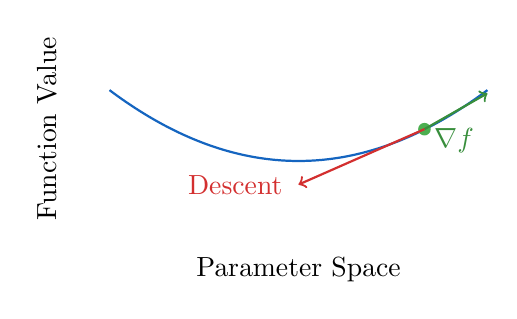
\begin{tikzpicture}[scale=0.8]
            % Draw function curve
            \draw[thick, approxmain] (-3,2) .. controls (-1,0.5) and (1,0.5) .. (3,2);

            % Point on curve
            \fill[targetcolor] (2,1.38) circle (0.1);

            % Gradient arrow
            \draw[->, thick, gradientcolor] (2,1.38) -- (3, 1.95);
            \node[gradientcolor, right] at (2,1.2) {$\nabla f$};

            % Descent direction
            \draw[->, thick, errorcolor] (2,1.38) -- (0,0.5);
            \node[errorcolor, left] at (-0.1,0.5) {Descent};

            \node[below] at (0,-0.5) {Parameter Space};
            \node[left, rotate=90] at (-4,3) {Function Value};
        \end{tikzpicture}
    \end{center}

    \begin{block}<4->{Gradient Descent Update}
        \begin{align}
            \mathbf{w}_{t+1} = \mathbf{w}_t - \alpha \nabla f(\mathbf{w}_t)
        \end{align}
        where $\alpha$ is the \textcolor{approxaccent}{\textbf{learning rate}}
    \end{block}
\end{frame}

\begin{frame}
    \frametitle{Gradient Descent Intuition}

    \begin{block}{What is a Gradient?}
        \begin{itemize}
            \item \textcolor{gradientcolor}{\textbf{Slope}} of a function at a specific point
            \item Points in direction of \textcolor{gradientcolor}{\textbf{steepest increase}}
            \item For function $f(\mathbf{w})$: $\nabla f(\mathbf{w}) = \left( \frac{\partial f}{\partial w_1}, \ldots, \frac{\partial f}{\partial w_d} \right)^T$
        \end{itemize}
    \end{block}

    \begin{block}<2->{Gradient Descent Update}
        $$\mathbf{w}_{t+1} = \mathbf{w}_t - \alpha \nabla f(\mathbf{w}_t)$$
        where $\alpha$ is the \textcolor{approxaccent}{\textbf{learning rate}}
    \end{block}
\end{frame}

\begin{frame}
    \frametitle{Example: Gradient Calculation - Setup}

    \begin{block}{Function: $f(x,y) = 0.5x^2 + y^2$}
        Find the gradient at point $(x=10, y=10)$
    \end{block}

    \begin{block}{Step 1: Partial Derivatives}
        \begin{align*}
            \frac{\partial f}{\partial x} &= x \\
            \frac{\partial f}{\partial y} &= 2y
        \end{align*}
    \end{block}

\end{frame}

\begin{frame}
    \frametitle{Example: Gradient Calculation - Vector Form}

    \begin{block}{Step 2: Gradient Vector}
        \begin{align*}
            \nabla f(x,y) = \begin{bmatrix} x \\ 2y \end{bmatrix}
        \end{align*}
    \end{block}

    \begin{block}{Step 3: Evaluate at $(10,10)$}
        \begin{align*}
            \nabla f(10,10) = \begin{bmatrix} 10 \\ 20 \end{bmatrix}
        \end{align*}
    \end{block}

\end{frame}

\begin{frame}
    \frametitle{Activity: 2D Gradient Descent Practice}

    \begin{alertblock}{Your Turn}
        Execute two steps of gradient descent starting from $(x_0, y_0) = (2, 3)$ with $\alpha = 0.1$ for:
        $$f(x,y) = x^2 + 2y^2 - 4x - 6y + 10$$

        \vspace{0.5em}
        \textbf{Steps to follow:}
        \begin{enumerate}
            \item Find the gradient $\nabla f(x,y)$
            \item Calculate $(x_1, y_1)$ after first step
            \item Calculate $(x_2, y_2)$ after second step
        \end{enumerate}
    \end{alertblock}

\end{frame}

\begin{frame}
    \frametitle{Solution: Step 1 - Gradient Calculation}

    \begin{block}{Gradient of $f(x,y) = x^2 + 2y^2 - 4x - 6y + 10$}
        Taking partial derivatives:
        \begin{align}
            \frac{\partial f}{\partial x} &= 2x - 4 \\
            \frac{\partial f}{\partial y} &= 4y - 6
        \end{align}
    \end{block}

    \begin{block}{Gradient Vector}
        $$\nabla f(x,y) = \begin{bmatrix} 2x - 4 \\ 4y - 6 \end{bmatrix}$$
    \end{block}

\end{frame}

\begin{frame}
    \frametitle{Solution: Step 2 - First Iteration}

    \begin{block}{Starting Point: $(x_0, y_0) = (2, 3)$}
        Evaluate gradient at $(2,3)$:
        $$\nabla f(2,3) = \begin{bmatrix} 2(2) - 4 \\ 4(3) - 6 \end{bmatrix} = \begin{bmatrix} 0 \\ 6 \end{bmatrix}$$
    \end{block}

    \begin{block}{Update Rule: $\theta_{new} = \theta_{old} - \alpha \nabla f(\theta_{old})$}
        $$\begin{bmatrix} x_1 \\ y_1 \end{bmatrix} = \begin{bmatrix} 2 \\ 3 \end{bmatrix} - 0.1 \begin{bmatrix} 0 \\ 6 \end{bmatrix} = \begin{bmatrix} 2.0 \\ 2.4 \end{bmatrix}$$
    \end{block}

\end{frame}

\begin{frame}
    \frametitle{Solution: Step 3 - Second Iteration}

    \begin{block}{Starting Point: $(x_1, y_1) = (2.0, 2.4)$}
        Evaluate gradient at $(2.0, 2.4)$:
        $$\nabla f(2.0,2.4) = \begin{bmatrix} 2(2.0) - 4 \\ 4(2.4) - 6 \end{bmatrix} = \begin{bmatrix} 0 \\ 3.6 \end{bmatrix}$$
    \end{block}

    \begin{block}{Second Update}
        $$\begin{bmatrix} x_2 \\ y_2 \end{bmatrix} = \begin{bmatrix} 2.0 \\ 2.4 \end{bmatrix} - 0.1 \begin{bmatrix} 0 \\ 3.6 \end{bmatrix} = \begin{bmatrix} 2.0 \\ 2.04 \end{bmatrix}$$
    \end{block}

\end{frame}

\subsection{Stochastic Gradient Descent in RL}

\begin{frame}
    \frametitle{Why SGD in Reinforcement Learning?}

    \begin{block}{The Challenge}
        In RL, we want to learn value functions $v_\pi(s)$ or $q_\pi(s,a)$ but:
        \begin{itemize}
            \item We can't store a table for every state
            \item We need \textcolor{approxmain}{\textbf{function approximation}}
        \end{itemize}
    \end{block}

    \begin{block}<2->{Function Approximation}
        Represent value function with parameters: $\hat{v}(s,\mathbf{w})$
        \begin{itemize}
            \item<2-> $\mathbf{w}$ = weight vector (parameters)
            \item<3-> Could be linear: $\hat{v}(s,\mathbf{w}) = \mathbf{w}^T \mathbf{x}(s)$
            \item<4-> Or non-linear: neural networks, etc.
        \end{itemize}
    \end{block}

    \visible<5->{
        \begin{alertblock}{Goal}
            Find weights $\mathbf{w}$ that make $\hat{v}(s,\mathbf{w}) \approx v_\pi(s)$ for all states
        \end{alertblock}
    }
\end{frame}

\begin{frame}
    \frametitle{From Supervised Learning to RL}

    \begin{block}{Supervised Learning Setting}
        \begin{itemize}
            \item Have training data: $(x_1, y_1), (x_2, y_2), \ldots, (x_n, y_n)$
            \item Know true labels $y_i$
            \item Minimize loss: $\sum_i L(f(x_i), y_i)$
        \end{itemize}
    \end{block}

    \begin{block}<2->{RL Setting (if we had true values)}
        \begin{itemize}
            \item<2-> Training data: $(s_1, v_\pi(s_1)), (s_2, v_\pi(s_2)), \ldots$
            \item<3-> Minimize: $\sum_i [v_\pi(s_i) - \hat{v}(s_i,\mathbf{w})]^2$
            \item<4-> Use gradient descent to find optimal $\mathbf{w}$
        \end{itemize}
    \end{block}

    \visible<5->{
        \begin{alertblock}{The Problem}
            We don't know the true values $v_\pi(s_i)$! That's what we're trying to learn!
        \end{alertblock}
    }
\end{frame}

\begin{frame}
    \frametitle{SGD for Value Function Approximation}

    \begin{block}<1->{Assumptions}
        \begin{itemize}
            \item<1-> Approximate value function $\hat{v}(s,\mathbf{w})$ is \textcolor{gradientcolor}{\textbf{differentiable}}
            \item<2-> Observe samples $s_t \mapsto v_\pi(s_t)$ (state and true value)
            \item<3-> States appear according to distribution $\mu$
        \end{itemize}
    \end{block}

    \begin{block}<2->{Gradient of Squared Error}
            $$\nabla \left[ v_\pi(s_t) - \hat{v}(s_t,\mathbf{w}) \right]^2 = -2 \left[ v_\pi(s_t) - \hat{v}(s_t,\mathbf{w}) \right] \nabla\hat{v}(s_t,\mathbf{w})$$
    \end{block}

    \begin{block}<3->{SGD Update Rule}
        $$\mathbf{w}_{t+1} = \mathbf{w}_t + \alpha \left[ v_\pi(s_t) - \hat{v}(s_t,\mathbf{w}_t) \right] \nabla\hat{v}(s_t,\mathbf{w}_t)$$
    \end{block}
\end{frame}

\begin{frame}
    \frametitle{SGD for Value Function Approximation}

    \begin{block}{Gradient of Squared Error}
            $$\nabla \left[ v_\pi(s_t) - \hat{v}(s_t,\mathbf{w}) \right]^2 = -2 \left[ v_\pi(s_t) - \hat{v}(s_t,\mathbf{w}) \right] \nabla\hat{v}(s_t,\mathbf{w})$$
    \end{block}

    \begin{block}{SGD Update Rule}
        $$\mathbf{w}_{t+1} = \mathbf{w}_t + \alpha \left[ v_\pi(s_t) - \hat{v}(s_t,\mathbf{w}_t) \right] \nabla\hat{v}(s_t,\mathbf{w}_t)$$
    \end{block}

    \visible<2->{
        \begin{center}
            \textcolor{approxmain}{\textbf{Problem}: We don't know $v_\pi(s_t)$!}
        \end{center}
    }
\end{frame}

\begin{frame}
    \frametitle{The SGD Update Rule Explained}

    \begin{block}{Standard SGD Update}
        $$\mathbf{w}_{t+1} = \mathbf{w}_t + \alpha \left[ v_\pi(s_t) - \hat{v}(s_t,\mathbf{w}_t) \right] \nabla\hat{v}(s_t,\mathbf{w}_t)$$
    \end{block}

    \begin{block}<2->{Breaking it Down}
        \begin{itemize}
            \item<2-> $v_\pi(s_t) - \hat{v}(s_t,\mathbf{w}_t)$ = \textcolor{errorcolor}{\textbf{prediction error}}
            \item<3-> $\nabla\hat{v}(s_t,\mathbf{w}_t)$ = \textcolor{gradientcolor}{\textbf{gradient}} (direction of steepest increase)
            \item<4-> $\alpha$ = \textcolor{targetcolor}{\textbf{learning rate}} (step size)
        \end{itemize}
    \end{block}

    \begin{block}<5->{Intuition}
        \begin{itemize}
            \item<5-> If $\hat{v}(s_t,\mathbf{w}_t) < v_\pi(s_t)$: error is positive $\Rightarrow$ increase $\mathbf{w}$ in gradient direction
            \item<6-> If $\hat{v}(s_t,\mathbf{w}_t) > v_\pi(s_t)$: error is negative $\Rightarrow$ decrease $\mathbf{w}$ in gradient direction
        \end{itemize}
    \end{block}
\end{frame}

\begin{frame}
    \frametitle{Using Target Approximations}

    \begin{block}<1->{Solution: Unbiased Target Estimates}
        Replace true value $v_\pi(s_t)$ with unbiased estimate $U_t$
    \end{block}

    \begin{block}<2->{General SGD Update}
        $$\mathbf{w}_{t+1} = \mathbf{w}_t + \alpha \left[ U_t - \hat{v}(s_t,\mathbf{w}_t) \right] \nabla\hat{v}(s_t,\mathbf{w}_t)$$
    \end{block}

    \begin{block}<3->{Target Choices}
        \begin{itemize}
            \item<3-> \textbf{Monte Carlo}: $U_t = G_t$ (sample return)
            \item<4-> \textbf{TD(0)}: $U_t = r_{t+1} + \gamma\hat{v}(s_{t+1},\mathbf{w}_t)$
        \end{itemize}
    \end{block}

    \visible<5->{
        \begin{alertblock}{Key Insight}
            The target $U_t$ must be an \textcolor{targetcolor}{\textbf{unbiased estimate}} of $v_\pi(s_t)$ for convergence guarantees
        \end{alertblock}
    }
\end{frame}

\begin{frame}
    \frametitle{Target Approximations: Detailed Explanation}

    \begin{block}{Why Different Targets?}
        Each target $U_t$ represents a different way to estimate $v_\pi(s_t)$:
    \end{block}

    \begin{block}<2->{Monte Carlo Target: $U_t = G_t$}
        \begin{itemize}
            \item<2-> $G_t = r_{t+1} + \gamma r_{t+2} + \gamma^2 r_{t+3} + \ldots$ (actual return)
            \item<3-> \textcolor{stfxblue}{\textbf{Pro}}: Unbiased estimate of $v_\pi(s_t)$
            \item<4-> \textcolor{red}{\textbf{Con}}: High variance, need complete episodes
        \end{itemize}
    \end{block}

    \begin{block}<5->{TD(0) Target: $U_t = r_{t+1} + \gamma\hat{v}(s_{t+1},\mathbf{w}_t)$}
        \begin{itemize}
            \item<5-> Bootstrap from current estimate of next state
            \item<6-> \textcolor{stfxblue}{\textbf{Pro}}: Lower variance, online updates
            \item<7-> \textcolor{red}{\textbf{Con}}: Biased (depends on current approximation)
        \end{itemize}
    \end{block}
\end{frame}

\begin{frame}
    \frametitle{Convergence Properties}

    \begin{block}{When Does SGD Converge?}
        For convergence, we need:
        \begin{enumerate}
            \item<1-> Target $U_t$ is an \textcolor{targetcolor}{\textbf{unbiased estimate}} of $v_\pi(s_t)$
            \item<2-> Learning rate conditions: $\sum_t \alpha_t = \infty$ and $\sum_t \alpha_t^2 < \infty$
            \item<3-> Function approximator is \textcolor{gradientcolor}{\textbf{differentiable}}
        \end{enumerate}
    \end{block}

    \begin{block}<4->{Convergence Guarantees}
        \begin{itemize}
            \item<4-> \textcolor{stfxblue}{\textbf{Monte Carlo}}: Converges to global optimum (unbiased target)
            \item<5-> \textcolor{orange}{\textbf{TD methods}}: May not converge (biased target)
            \item<6-> \textcolor{blue}{\textbf{Practice}}: TD methods often work well despite theory
        \end{itemize}
    \end{block}

    \visible<7->{
        \begin{alertblock}{Key Takeaway}
            There's a bias-variance tradeoff in choosing targets for SGD
        \end{alertblock}
    }
\end{frame}

% Section: Algorithms
\section{Gradient-Based Algorithms}

\subsection{Gradient Monte Carlo}

\begin{frame}
    \frametitle{Gradient Monte Carlo Method}

    \begin{algorithm}[H]
        \caption{Gradient Monte Carlo for Value Function Approximation}
        \begin{algorithmic}[1]
            \State \textbf{Input}: Policy $\pi$, number of episodes $N$, step size $\alpha \in (0,1]$
            \State \textbf{Initialize}: $\mathbf{w} \in \mathbb{R}^d$ arbitrarily (e.g., $\mathbf{w} = \mathbf{0}$)
            \For{$N$ episodes}
                \State Generate episode using $\pi$: $S_0, A_0, R_1, S_1, \ldots, S_{T-1}, A_{T-1}, R_T$
                \For{each step $t = 0, 1, \ldots, T-1$}
                    \State $\mathbf{w} \leftarrow \mathbf{w} + \alpha[G_t - \hat{v}(S_t,\mathbf{w})]\nabla\hat{v}(S_t,\mathbf{w})$
                \EndFor
            \EndFor
        \end{algorithmic}
    \end{algorithm}

    \begin{block}<2->{Key Features}
        \begin{itemize}
            \item<2-> Uses \textcolor{targetcolor}{\textbf{actual returns}} $G_t$ as targets
            \item<3-> \textcolor{targetcolor}{\textbf{Unbiased}} - guaranteed convergence to local optimum
            \item<4-> Requires \textcolor{errorcolor}{\textbf{complete episodes}}
        \end{itemize}
    \end{block}
\end{frame}

\subsection{Semi-Gradient TD(0)}

\begin{frame}
    \frametitle{Semi-Gradient TD(0)}

    \begin{algorithm}[H]
        \caption{Semi-Gradient TD(0)}
        \begin{algorithmic}[1]
            \State \textbf{Input}: Policy $\pi$, step size $\alpha \in (0,1]$
            \State \textbf{Initialize}: $\mathbf{w} \in \mathbb{R}^d$ arbitrarily
            \Repeat
                \State Initialize $S$
                \Repeat
                    \State $A \leftarrow \pi(\cdot|S)$
                    \State Take action $A$, observe $R, S'$
                    \State $\mathbf{w} \leftarrow \mathbf{w} + \alpha[R + \gamma\hat{v}(S',\mathbf{w}) - \hat{v}(S,\mathbf{w})]\nabla\hat{v}(S,\mathbf{w})$
                    \State $S \leftarrow S'$
                \Until{$S$ is terminal}
            \Until{convergence}
        \end{algorithmic}
    \end{algorithm}
\end{frame}

\begin{frame}
    \frametitle{Semi-Gradient TD(0)}

    \begin{block}{Why "Semi-Gradient"?}
        \begin{itemize}
            \item<2-> Target includes $\hat{v}(S',\mathbf{w})$ which depends on $\mathbf{w}$
            \item<3-> We ignore gradient w.r.t. target: \textcolor{errorcolor}{\textbf{not true gradient}}
            \item<4-> Still converges but to different solution than true gradient
        \end{itemize}
    \end{block}
\end{frame}

% Section: On-Policy Control
\section{On-Policy Control}

\subsection{Action-Value Function Approximation}

\begin{frame}
    \frametitle{From State Values to Action Values}

    \begin{block}<1->{Extending to Control}
        \begin{itemize}
            \item<1-> Need action-value function: $\hat{q}(s,a,\mathbf{w})$ instead of $\hat{v}(s,\mathbf{w})$
            \item<2-> Same principles apply with weight vector $\mathbf{w}$
        \end{itemize}
    \end{block}

    \begin{block}<2->{General Update for Action Values}
            $$\mathbf{w}_{t+1} = \mathbf{w}_t + \alpha \left[ U_t - \hat{q}(S_t,A_t,\mathbf{w}_t) \right] \nabla\hat{q}(S_t,A_t,\mathbf{w}_t)$$
    \end{block}

    \begin{block}<3->{SARSA Target}
        For one-step SARSA: $U_t = R_{t+1} + \gamma\hat{q}(S_{t+1},A_{t+1},\mathbf{w}_t)$
    \end{block}

    \begin{block}<4->{Policy Improvement}
        \begin{itemize}
            \item<4-> Compute $\hat{q}(s,a,\mathbf{w})$ for all actions $a$
            \item<5-> Use $\epsilon$-greedy: $a^* = \arg\max_a \hat{q}(s,a,\mathbf{w})$
        \end{itemize}
    \end{block}
\end{frame}

\subsection{Semi-Gradient SARSA}

\begin{frame}
    \frametitle{Semi-Gradient SARSA Algorithm}

    \begin{algorithm}[H]
        \begin{algorithmic}[1]
            \State \textbf{Input}: $\hat{q}: \mathcal{S} \times \mathcal{A} \times \mathbb{R}^d \rightarrow \mathbb{R}$, step size $\alpha$, $\epsilon > 0$
            \State \textbf{Initialize}: $\mathbf{w} \in \mathbb{R}^d$ arbitrarily
            \Repeat
                \State Initialize $S$
                \State $A \leftarrow \epsilon\text{-greedy}(\hat{q}(S,\cdot,\mathbf{w}))$
                \Repeat
                    \State Take action $A$, observe $R, S'$
                    \If{$S'$ is terminal}
                        \State $\mathbf{w} \leftarrow \mathbf{w} + \alpha[R - \hat{q}(S,A,\mathbf{w})]\nabla\hat{q}(S,A,\mathbf{w})$
                        \State \textbf{break}
                    \EndIf
                    \State $A' \leftarrow \epsilon\text{-greedy}(\hat{q}(S',\cdot,\mathbf{w}))$
                    \State $\mathbf{w} \leftarrow \mathbf{w} + \alpha[R + \gamma\hat{q}(S',A',\mathbf{w}) - \hat{q}(S,A,\mathbf{w})]\nabla\hat{q}(S,A,\mathbf{w})$
                    \State $S \leftarrow S'$, $A \leftarrow A'$
                \Until{$S$ is terminal}
            \Until{convergence}
        \end{algorithmic}
    \end{algorithm}
\end{frame}

% Section: Function Approximation Methods
\section{Function Approximation Methods}

\subsection{State Aggregation}

\begin{frame}
    \frametitle{State Aggregation}

    \begin{block}<1->{Basic Idea}
        \begin{itemize}
            \item<1-> Group \textcolor{statecolor}{\textbf{similar states}} together
            \item<2-> Assign \textcolor{approxaccent}{\textbf{same value}} to states in same group
            \item<3-> Simplest form of function approximation
        \end{itemize}
    \end{block}

    \begin{center}
        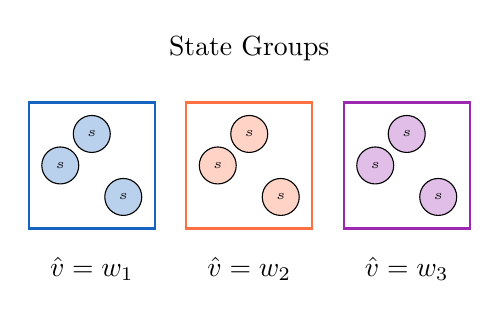
\begin{tikzpicture}[scale=0.8]
            % Draw state groups
            \draw[thick, approxmain] (-2,-1) rectangle (0,1);
            \draw[thick, approxaccent] (0.5,-1) rectangle (2.5,1);
            \draw[thick, statecolor] (3,-1) rectangle (5,1);

            % States within groups
            \foreach \x/\y in {-1.5/0, -1/0.5, -0.5/-0.5} {
                \node[circle, fill=approxmain!30, draw] at (\x,\y) {\tiny $s$};
            }
            \foreach \x/\y in {1/0, 1.5/0.5, 2/-0.5} {
                \node[circle, fill=approxaccent!30, draw] at (\x,\y) {\tiny $s$};
            }
            \foreach \x/\y in {3.5/0, 4/0.5, 4.5/-0.5} {
                \node[circle, fill=statecolor!30, draw] at (\x,\y) {\tiny $s$};
            }

            % Values
            \node[below] at (-1,-1.3) {$\hat{v} = w_1$};
            \node[below] at (1.5,-1.3) {$\hat{v} = w_2$};
            \node[below] at (4,-1.3) {$\hat{v} = w_3$};

            \node[above] at (1.5,1.5) {State Groups};
        \end{tikzpicture}
    \end{center}
\end{frame}

\begin{frame}
    \frametitle{State Aggregation}

    \begin{block}{Basic Idea}
        \begin{itemize}
            \item Group \textcolor{statecolor}{\textbf{similar states}} together
            \item Assign \textcolor{approxaccent}{\textbf{same value}} to states in same group
            \item Simplest form of function approximation
        \end{itemize}
    \end{block}

    \begin{alertblock}<1->{Limitations}
        \begin{itemize}
            \item<1-> Works only for \textcolor{errorcolor}{\textbf{simple problems}}
            \item<2-> Hard to define good groupings
            \item<3-> No generalization within groups
        \end{itemize}
    \end{alertblock}
\end{frame}

\subsection{Linear Function Approximation}

\begin{frame}
    \frametitle{Linear Methods}

    \begin{block}<1->{Linear Approximation}
        $$\hat{v}(s,\mathbf{w}) = \mathbf{w}^T\mathbf{x}(s) = \sum_{i=1}^d w_i x_i(s)$$
        where $\mathbf{x}(s) = (x_1(s), x_2(s), \ldots, x_d(s))^T$ is the \textcolor{featurecolor}{\textbf{feature vector}}
    \end{block}

    \begin{block}<2->{Key Advantage: Simple Gradient}
        $$\nabla\hat{v}(s,\mathbf{w}) = \mathbf{x}(s)$$
    \end{block}

    \begin{block}<3->{Linear SGD Update}

        $$\mathbf{w}_{t+1} = \mathbf{w}_t + \alpha \left[ U_t - \hat{v}(S_t,\mathbf{w}_t) \right] \mathbf{x}(S_t)$$

    \end{block}

    \visible<4->{
        \begin{center}
            \textcolor{approxmain}{\textbf{Challenge}: How to construct good features?}
        \end{center}
    }
\end{frame}

\begin{frame}
    \frametitle{Feature Construction Example}

    \begin{block}<1->{Problem Setup}
        State has two dimensions: $s = (s_1, s_2)$ where $s_1, s_2 \in \mathbb{R}$
    \end{block}

    \begin{block}<2->{Simple Linear Features}
        $\mathbf{x}(s) = [s_1, s_2]^T$
        \begin{itemize}
            \item<3-> \textcolor{errorcolor}{\textbf{Problem}}: Cannot represent interactions between $s_1$ and $s_2$
            \item<4-> \textcolor{errorcolor}{\textbf{Problem}}: If $s_1 = s_2 = 0$, then $\hat{v}(s,\mathbf{w}) = 0$ always
        \end{itemize}
    \end{block}

    \begin{block}<5->{Polynomial Features}
        $\mathbf{x}(s) = [1, s_1, s_2, s_1s_2]^T$
        \begin{itemize}
            \item<6-> \textcolor{targetcolor}{\textbf{Benefit}}: Can represent interactions
        \end{itemize}
    \end{block}

    \begin{block}<8->{Higher-Order Polynomial}
        $\mathbf{x}(s) = [1, s_1, s_2, s_1s_2, s_1^2, s_2^2, s_1^2s_2, s_1s_2^2, s_1^2s_2^2]^T$
    \end{block}
\end{frame}

\end{document}
